\documentclass{ximera}

\newcommand{\RR}{\mathbb R}
\renewcommand{\d}{\,d}
\newcommand{\dd}[2][]{\frac{d #1}{d #2}}
\renewcommand{\l}{\ell}
\newcommand{\ddx}{\frac{d}{dx}}
\newcommand{\dfn}{\textbf}
\newcommand{\eval}[1]{\bigg[ #1 \bigg]}


\begin{document}
\textbf{For problems 9--11,} consider the region:
\[
R = \{(x,y,z): 0\le x \le 1, \sqrt{x}\le y\le 1, 0 \le z \le 1-y\}
\]
\begin{image}[2in]
  \includegraphics{3DRectRegion.png}
\end{image}

\begin{problem}
  \textbf{Fill-in} the \textbf{limits of integration} to compute the volume:
  \pdfOnly{\[\int\qquad\int\qquad\int\qquad\d z \d y \d x\]}
  \begin{prompt}
  \[
  \int_{\answer{0}}^{\answer{1}}\int_{\answer{\sqrt{x}}}^{\answer{1}}\int_{\answer{0}}^{\answer{1-y}}\d z \d y \d x
  \]
  \end{prompt}
\end{problem}



\begin{problem}
  \textbf{Fill-in} the \textbf{limits of integration} to compute the volume:
  \pdfOnly{\[\int\qquad\int\qquad\int\qquad\d y \d z \d x\]}
  \begin{prompt}
  \[
  \int_{\answer{0}}^{\answer{1}}\int_{\answer{0}}^{\answer{1-\sqrt{x}}}\int_{\answer{\sqrt{x}}}^{\answer{1-z}}\d y \d z \d x
  \]
  \end{prompt}
\end{problem}

\begin{problem}
  \textbf{Fill-in} the \textbf{limits of integration} to compute the volume:
  \pdfOnly{\[\int\qquad\int\qquad\int\qquad\d x \d y \d z\]}
  \begin{prompt}
  \[
  \int_{\answer{0}}^{\answer{1}}\int_{\answer{0}}^{\answer{1-z}}\int_{\answer{0}}^{\answer{y^2}}\d x \d y \d z
  \]
  \end{prompt}
\end{problem}



\hrule


Consider the table of \textbf{gradient vectors} for a differentiable
function $F:\R^2\to\R$ given below:
\begin{image}
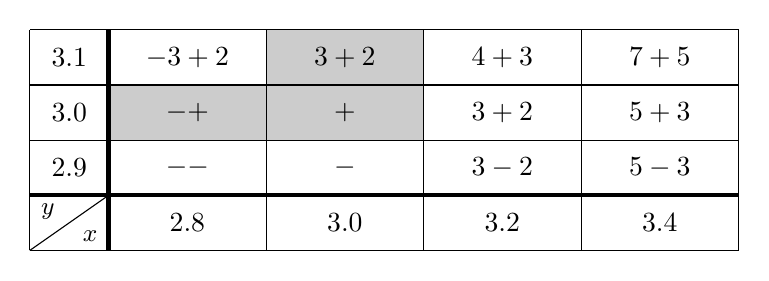
\begin{tikzpicture}[x=1cm,y=.7cm]

  \draw[fill=white!80!black]
  (1,2) -- (5,2) --(5,4) -- (3,4) -- (3,3) -- (1,3)--cycle;%(3,3) -- (7,3) --(7,2) -- (3,2)--cycle;
  
  \draw (0,0) grid [step=1] (1,4);
  \draw (3,4) -- (3,0);
  \draw (5,4) -- (5,0);
  \draw (7,4) -- (7,0);
  \draw (9,4) -- (9,0);
  
  \draw (0,0) -- (9,0);
  \draw (0,1) -- (9,1);
  \draw (0,2) -- (9,2);
  \draw (0,3) -- (9,3);
  \draw (0,4) -- (9,4);


  
  \draw[ultra thick] (0,1)--(9,1);
  \draw[ultra thick] (1,4)--(1,0);
  
  \draw (0,0) -- (1,1);
  %\node at (.9,.9) [below left,inner sep=1pt] {\small$y$};
  %\node at (0.1,.1) [above right,inner sep=1pt] {\small$x$};
  \node at (.1,.9) [below right,inner sep=1pt] {\small$y$};
  \node at (0.9,.1) [above left,inner sep=1pt] {\small$x$};
  
  
  %% x-values
  \node at (2,.5) {$2.8$};
  \node at (4,.5) {$3.0$};
  \node at (6,.5) {$3.2$};
  \node at (8,.5) {$3.4$};
  
  %% y-values
  \node at (0.5,1.5) {$2.9$};
  \node at (0.5,2.5) {$3.0$};
  \node at (0.5,3.5) {$3.1$};
  
  
  %% vectors
  %% top row
  \node at (2,3.5) {$-3\veci+2\vecj$};
  \node at (4,3.5) {$3\veci+2\vecj$};
  \node at (6,3.5) {$4\veci+3\vecj$};
  \node at (8,3.5) {$7\veci+5\vecj$};

  %% second row
  \node at (2,2.5) {$-\veci+\vecj$};
  \node at (4,2.5) {$\veci+\vecj$};
  \node at (6,2.5) {$3\veci+2\vecj$};
  \node at (8,2.5) {$5\veci+3\vecj$};
  
  %% bottom row
  \node at (2,1.5) {$-\veci-\vecj$};
  \node at (4,1.5) {$\veci-\vecj$};
  \node at (6,1.5) {$3\veci-2\vecj$};
  \node at (8,1.5) {$5\veci-3\vecj$};
  
\end{tikzpicture}
\end{image}


\begin{problem}
  Let $R$ be the \textbf{shaded region} above, and assume our gradient vectors
  are sampled in some reasonable way.  \textbf{Estimate} the surface
  area of $F$ over $R$.
  \begin{prompt}
    \[
    \text{Area}\approx\answer{\frac{2\sqrt{3}+\sqrt{14}}{50}}
    \]
  \end{prompt}
  \vfill
\end{problem}



\hrule

\begin{problem}
  Let $S = \{(x,y,z): x^2 +y^2 + z^2 \le 1\}$. Which quantity is \textbf{largest}?
  \begin{multipleChoice}
      \pdfOnly{\begin{multicols}{3}}
      \choice{$\iiint_S x^{3} \d V$}
      \choice{$\iiint_S x^{5} \d V$}
      \choice[correct]{Neither, they are equal.}
      \pdfOnly{\end{multicols}}
    \end{multipleChoice}
\end{problem}
\end{document}
